% % % % % % % % % % % % % % % % % % % % % % % % % % % % % % % % % % % % % % % % % % % %
%                                                                                     %
% Short Sectioned Assignment LaTeX Template Version 1.0 (5/5/12)                      %
% This template has been downloaded from: http://www.LaTeXTemplates.com               %
%                                                                                     %
% Original author:  Frits Wenneker (http://www.howtotex.com)                          %
%                                                                                     %
% Modified by: Fco Javier Sueza Rodríguez (fcosueza@disroot.org)                      %
%                                                                                     %
% Changes:                                                                            %
%	    - Custom Chapters, Sections and Subsections (titlesec package)                %
%           - Document type scrbook (oneside)                                         %
%           - Use babel-lang-spanish package and marvosym                             %
%           - Use hyperref, enumitem, tcolorbox and glossaries packages               %
%           - Use Time New Roman (mathptmx), Helvetic and Courier fonts               %
%                                                                                     %
% License: CC BY-NC-SA 3.0 (http://creativecommons.org/licenses/by-nc-sa/3.0/)        %
%                                                                                     %
% % % % % % % % % % % % % % % % % % % % % % % % % % % % % % % % % % % % % % % % % % % %

%-----------------------------------------------%
%	              Packages                  %
%-----------------------------------------------%

\documentclass[paper=a4, fontsize=11pt, oneside]{scrbook}

% ---- Text Input/Output ----- %

\usepackage[T1]{fontenc}
\usepackage[utf8]{inputenc}
\usepackage{mathptmx}
\usepackage[scaled=.92]{helvet}
\usepackage{courier}
\usepackage[indent=12pt]{parskip}

\usepackage{geometry}
\geometry{verbose,tmargin=3cm,bmargin=3cm,lmargin=2.6cm,rmargin=2.6cm}

% ---- Language ----- %

\usepackage[spanish]{babel}
\usepackage{marvosym}

% ---- Another packages ---- %

\usepackage{amsmath,amsfonts,amsthm}
\usepackage{graphics,graphicx}
\usepackage{titlesec}
\usepackage{fancyhdr}
\usepackage{tcolorbox}
\usepackage{hyperref}
\usepackage{enumitem}
\usepackage[automake]{glossaries}

%--------------------------------------------------------------------%
%                      Customizing Document                          %
%--------------------------------------------------------------------%


% ----------- Custom Chapters, Sections and Subsections -------------- %

\titleformat{\chapter}[display]
			{\bfseries\Huge}
			{Tema \ \thechapter} {0.5ex}
			{\vspace{1ex}\centering}

\titleformat{\section}[hang]
			{\bfseries\Large}
			{\thesection}{0.5em}{}

\titleformat{\subsection}[hang]
			{\bfseries\large}
			{\thesubsection}{0.5em}{}

\titleformat{\subsubsection}[hang]
			{\bfseries\large}
			{\thesubsubsection}{0.5em}{}

\hypersetup{
    colorlinks=true,
    linkcolor=black,
    urlcolor=magenta
}

% ------------------- Custom heaaders and footers ------------------- %

\pagestyle{fancyplain}

\fancyhead[]{}
\fancyfoot[L]{}
\fancyfoot[C]{}
\fancyfoot[R]{\thepage}

\renewcommand{\headrulewidth}{0pt} % Remove header underlines
\renewcommand{\footrulewidth}{0pt} % Remove footer underlines

\setlength{\headheight}{13.6pt} % Customize the height of the header

% --------- Numbering equations, figures and tables ----------------- %

\numberwithin{equation}{section} % Number equations within sections
\numberwithin{figure}{section} % Number figures within sections
\numberwithin{table}{section} % Number tables within sections

% ------------------------ New Commands ----------------------------- %

\newcommand{\horrule}[1]{\rule{\linewidth}{#1}} % Create horizontal rule command


%----------------------------------------------------------------------------------------
%	TÍTULO Y DATOS DEL ALUMNO
%----------------------------------------------------------------------------------------

\title{
\vspace{10ex}
\normalfont \normalsize
\huge \textbf{Tarea 2: Monetizando mi Web/Blog SEM}
}
\author{Francisco Javier Sueza Rodríguez}
\date{\normalsize\today}

%----------------------------------------------------------------------------------------
%                                     DOCUMENTO
%----------------------------------------------------------------------------------------
\begin{document}

\maketitle

\thispagestyle{empty}

\vspace{65ex}

\begin{center}
    \begin{tabular}{l l}
        \textbf{Centro}: & IES Aguadulce \\
        \textbf{Ciclo Formativo}: & Desarrollo Aplicaciones Web (Distancia)\\
        \textbf{Asignatura}: & Horas de Libre Configuración\\
        \textbf{Tema}: & Tema 2 -  Monetizando mi Web/Blog SEM\\
    \end{tabular}
\end{center}

\newpage

\tableofcontents

\vspace{30ex}

\listoffigures

\newpage

\section{Introducción}
En esta tarea vamos a realizar una campaña de Google Ads para monetizar nuestra Web. En mi caso, vamos a realizar una campaña para atraer clientes a nuestra empresa ficticia, SiteWISE, una empresa de desarrollo de páginas web ubicada en Granada.

Con la cuenta creada como se nos indica en la unidad, aspecto que no se va a cubrir en este documento ya que no se especifica en los ejercicios de la tarea, vamos a crear nuestra campaña con los requisitos pedidos en los siguientes ejercicios.

\section{Ejercicio 1}

\subsection{Enunciado}
Para la campaña debes seleccionar 4 palabras clave relevantes que tengan que ver con el producto o servicio que quieras  que ofrecer.

\subsection{Solución}
En primer lugar, vamos a seleccionar 4 palabras que usaremos en nuestra campaña relacionada con el servicio que vamos a ofrecer. En nuestro caso, vamos a elegir \textbf{desarrollo web}, \textbf{diseño web}, \textbf{e-commerce} y \textbf{programador web en Granada}, ya que estás palabras se ajustan perfectamente al servicio que vamos a ofrecer, que es el desarrollo de páginas web.

\section{Ejercicio 2}

\subsection{Enunciado}
Crea una campaña para la red de búsqueda, seleccionando como objetivo tráfico en la web (debes utilizar o tu web o el blog que creaste en la tarea1)  ponle un nombre que lo identifique y configúrala con los siguientes datos:

\begin{itemize}
    \item Selecciona como ubicación la ciudad o ciudades donde ofrezcas tus servicios.
    \item Dependiendo del servicio o el producto o si es una tienda física deberás programar el horario en los que se imprimirán los anuncios  ( pulsa en más ajuste abajo del todo para encontrar esta sección)
    \item Fecha de inicio ( debes decidirla tú, según cuando crees que será más adecuado iniciarla) fecha de finalización  el día 10 de enero.
    \item Utiliza alguna sugerencia de palabras claves (2) y las otras 2 inventadas por ti, debes utilizar concordancia de frase y exacta en alguna de ellas y explicar en qué casos se activará tu anuncio con las búsquedas que realice el usuario en función del tipo de concordancia que hayas puesto.
\end{itemize}

\subsection{Solución}
En este punto vamos a empezar a configurar nuestra campaña de Google Ads introduciendo algunos datos básicos. Los pasos que hemos seguido son los siguientes:

\begin{enumerate}
    \item En primer lugar, hemos pulsado en el botón \textit{Crear} que se encuentra en la parte superior izquierda de la interfaz de google y hemos seleccionado \textit{Campaña} para comenzar a crear nuestra campaña, como podemos ver en la siguiente captura.

    \begin{figure}[H]
        \centering
        \includegraphics[scale=0.28]{campana-crear.png}
        \caption{Comienzo de creación de la campaña de Google Ads}
    \end{figure}

    \item Una iniciada la creación, nos pide que introduzcamos el objetivo de nuestra campaña, que en nuestro caso es \textbf{generar tráfico web}, que es el que hemos seleccionado, como vemos en la siguiente captura.

    \begin{figure}[H]
        \centering
        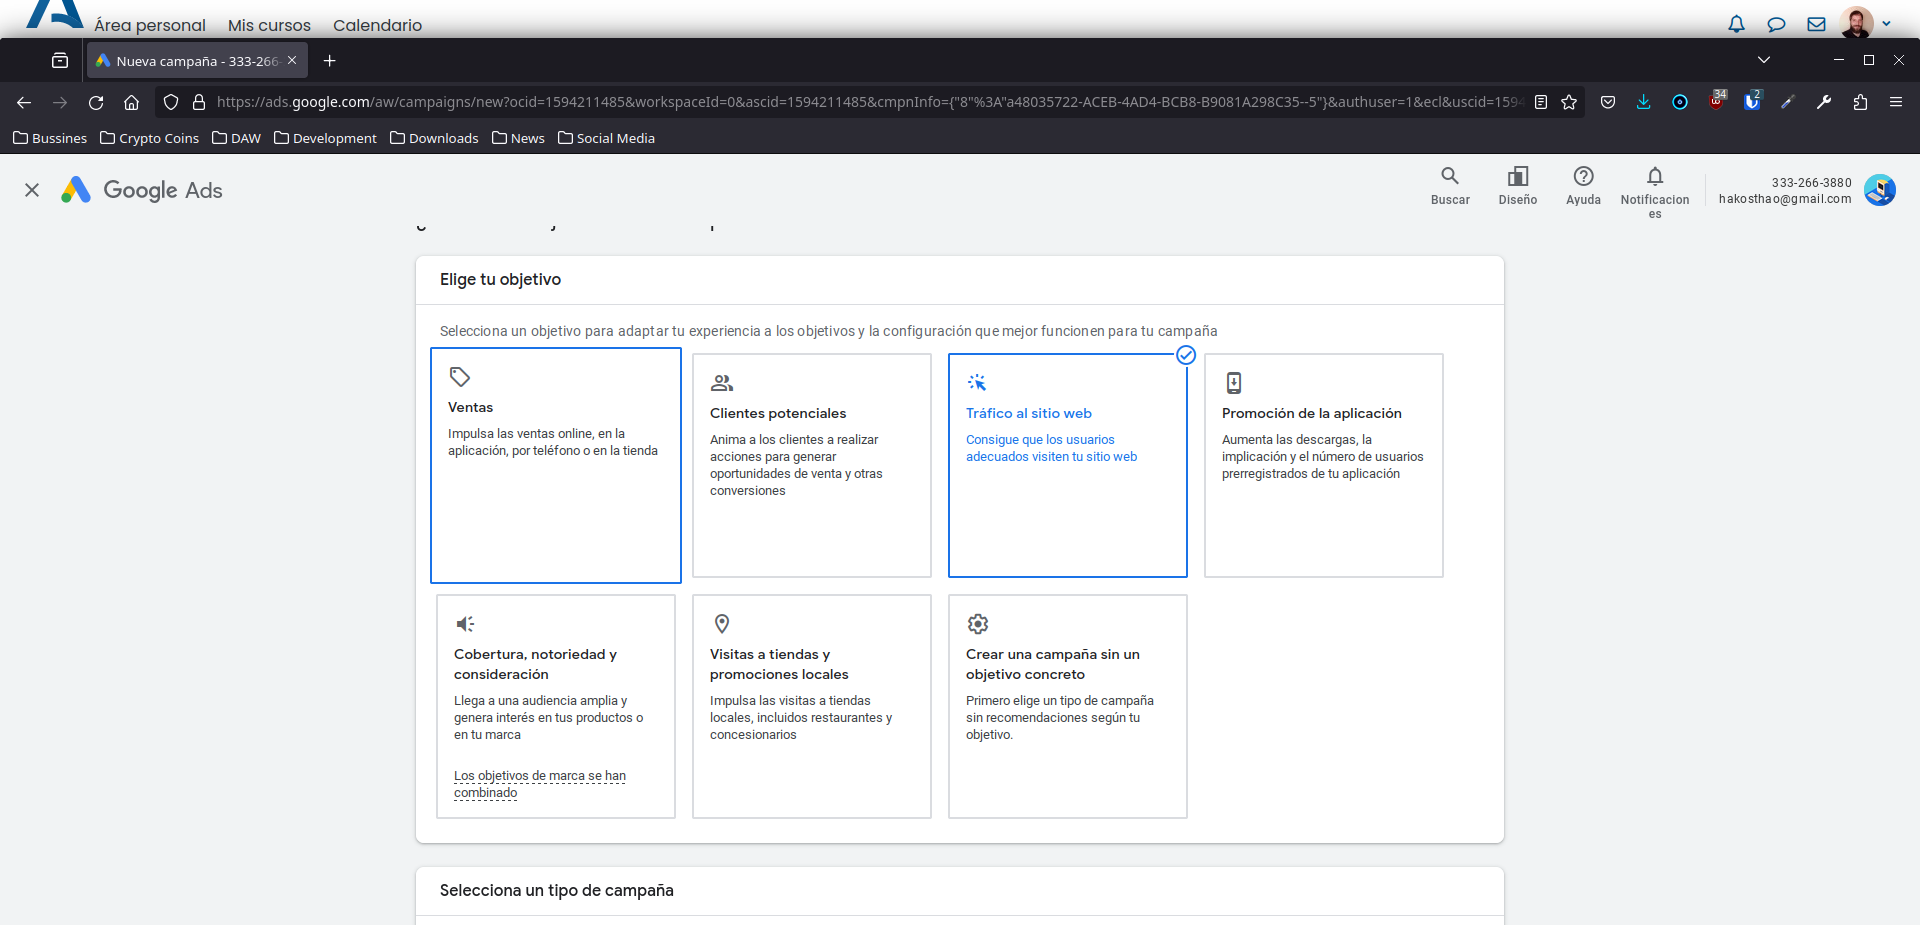
\includegraphics[scale=0.28]{Campana-obj.png}
        \caption{Selección del objetivo de la campaña}
    \end{figure}

    \item Una vez seleccionado nuestro objetivo, tenemos que seleccionar el tipo de campaña que vamos a crear. Tenemos diferentes opciones, como una campaña de búsqueda, máximo rendimiento, display, shopping, video o generación bajo demanda. Vamos a seleccionar \textbf{búsqueda}, ya que es el que nos interesa. También hay que tener en cuenta que tenemos un presupuesto limitado, por lo que es una de las campañas más básicas y también de las menos costosas.

    En la siguiente captura podemos ver la selección de esta opción.

    \begin{figure}[H]
        \centering
        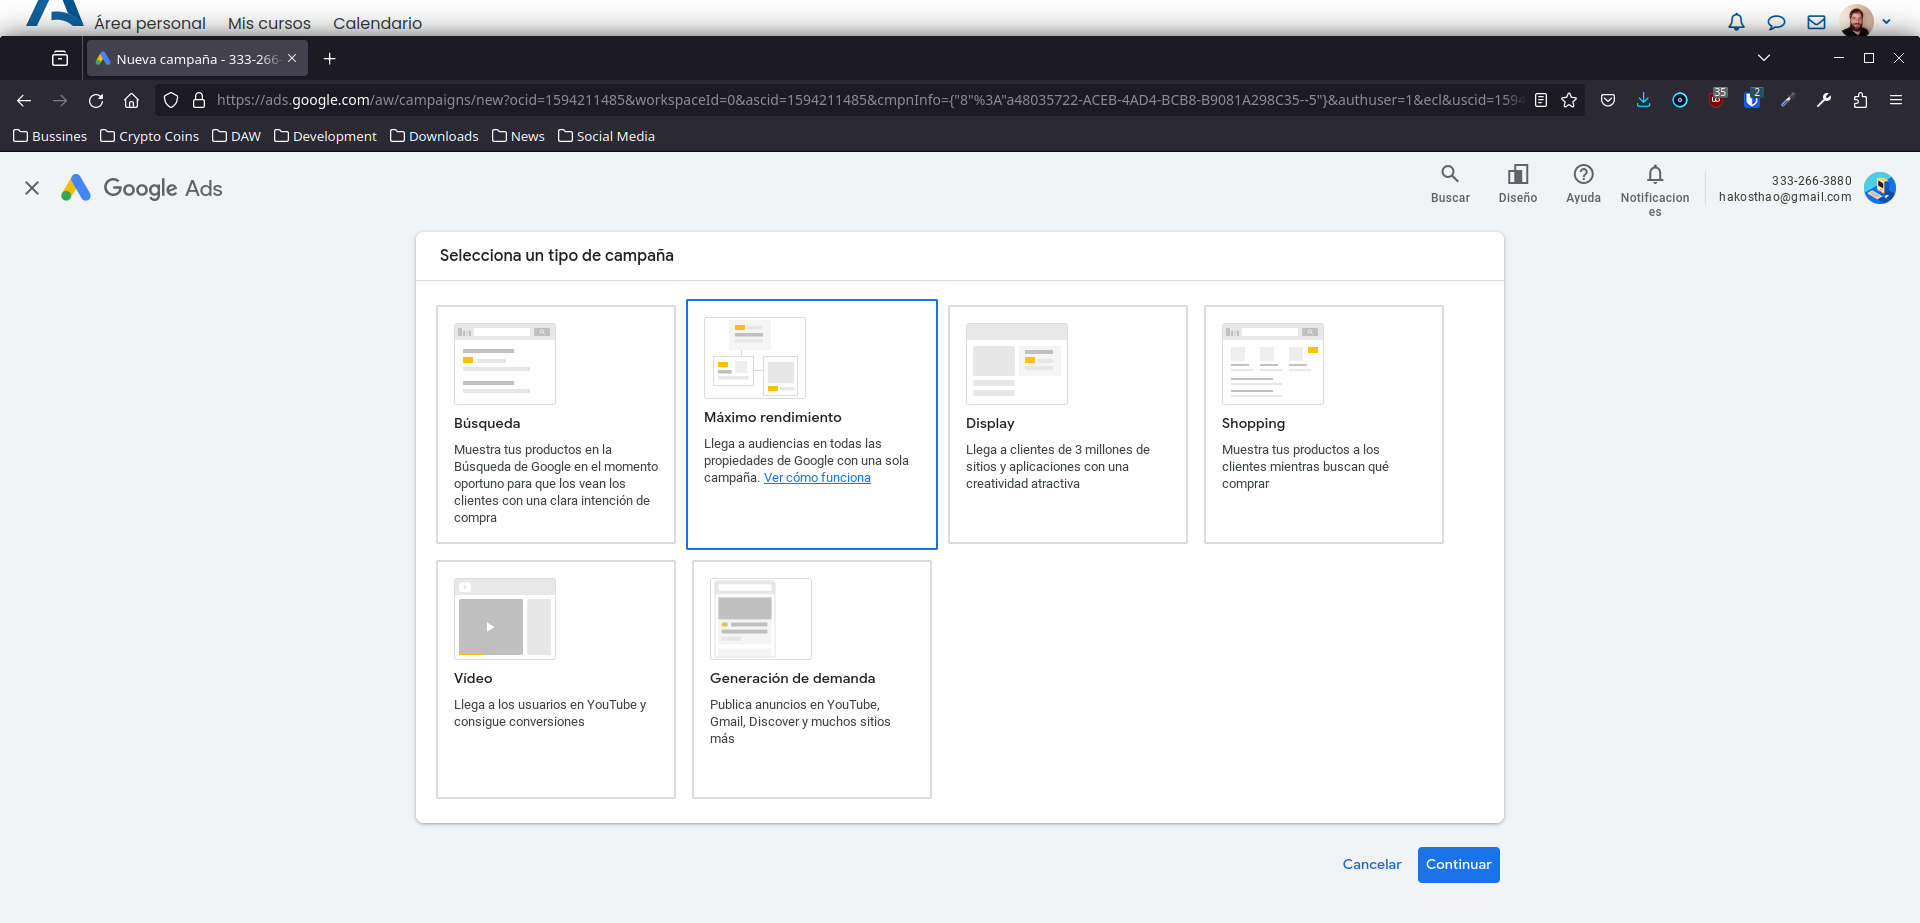
\includegraphics[scale=0.28]{Campana-tipo.png}
        \caption{Selección del tipo de campaña}
    \end{figure}

    \item Una vez seleccionado el tipo de de campaña, se nos mostrará un pantalla para que  introduzcamos la dirección web sobre el que queremos hacer la campaña. En nuestro caso es \href{https://sites.google.com/view/sitewise/inicio}{SiteWISE}, por lo que lo introducimos y seleccionamos la opción que se nos muestra en los objetivos de conversión web, es decir, las acciones que nos reportarán beneficio. Seleccionamos la opción \textbf{Vista de una página} y pulsamos en siguiente.

    \begin{figure}[H]
        \centering
        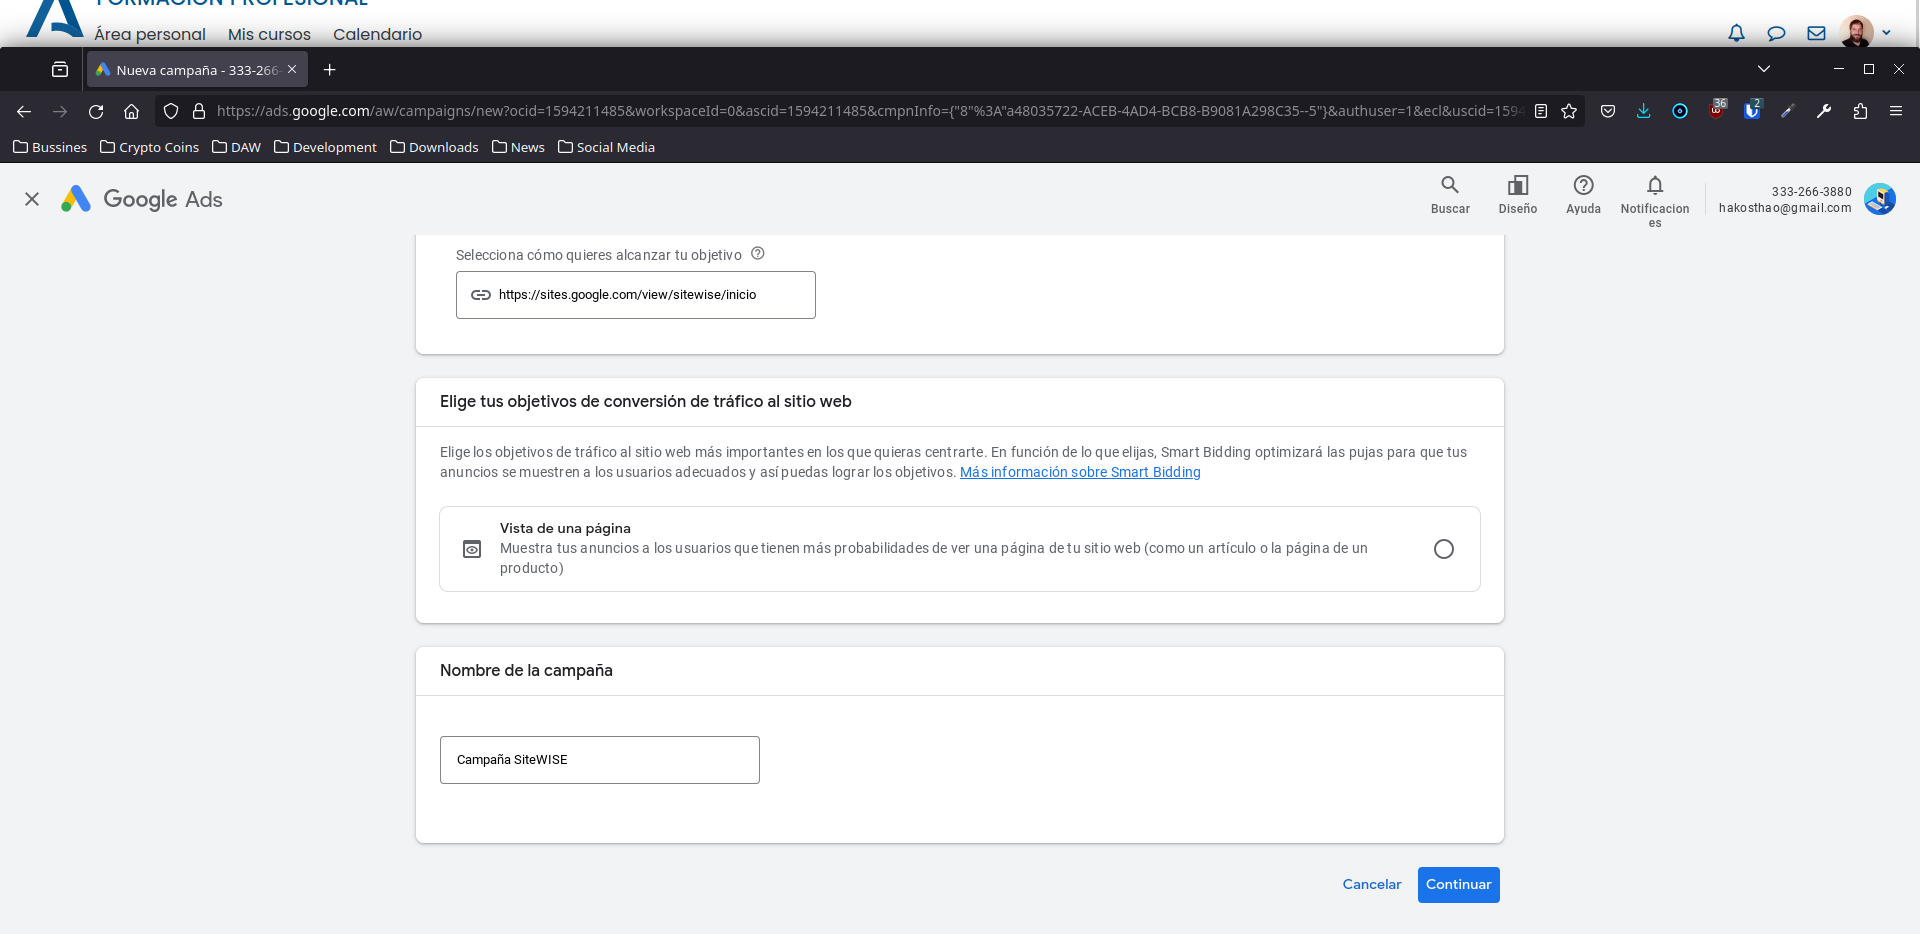
\includegraphics[scale=0.28]{Campana-web.png}
        \caption{Introducciónd de la dirección Web}
    \end{figure}

    \item Una vez introducidos estos datos, se nos mostrará una pantalla con las puja. En nuestro caso, hemos seleccionado la opción de \textbf{Clics}, para centrarnos en ellos.

    Podríamos también centrarnos en conversiones, que hayamos definido y que proporcionen valor a nuestro negocio, pero a nosotros nos vale con centrarnos en los clicks que realicen los usuarios.


     \begin{figure}[H]
        \centering
        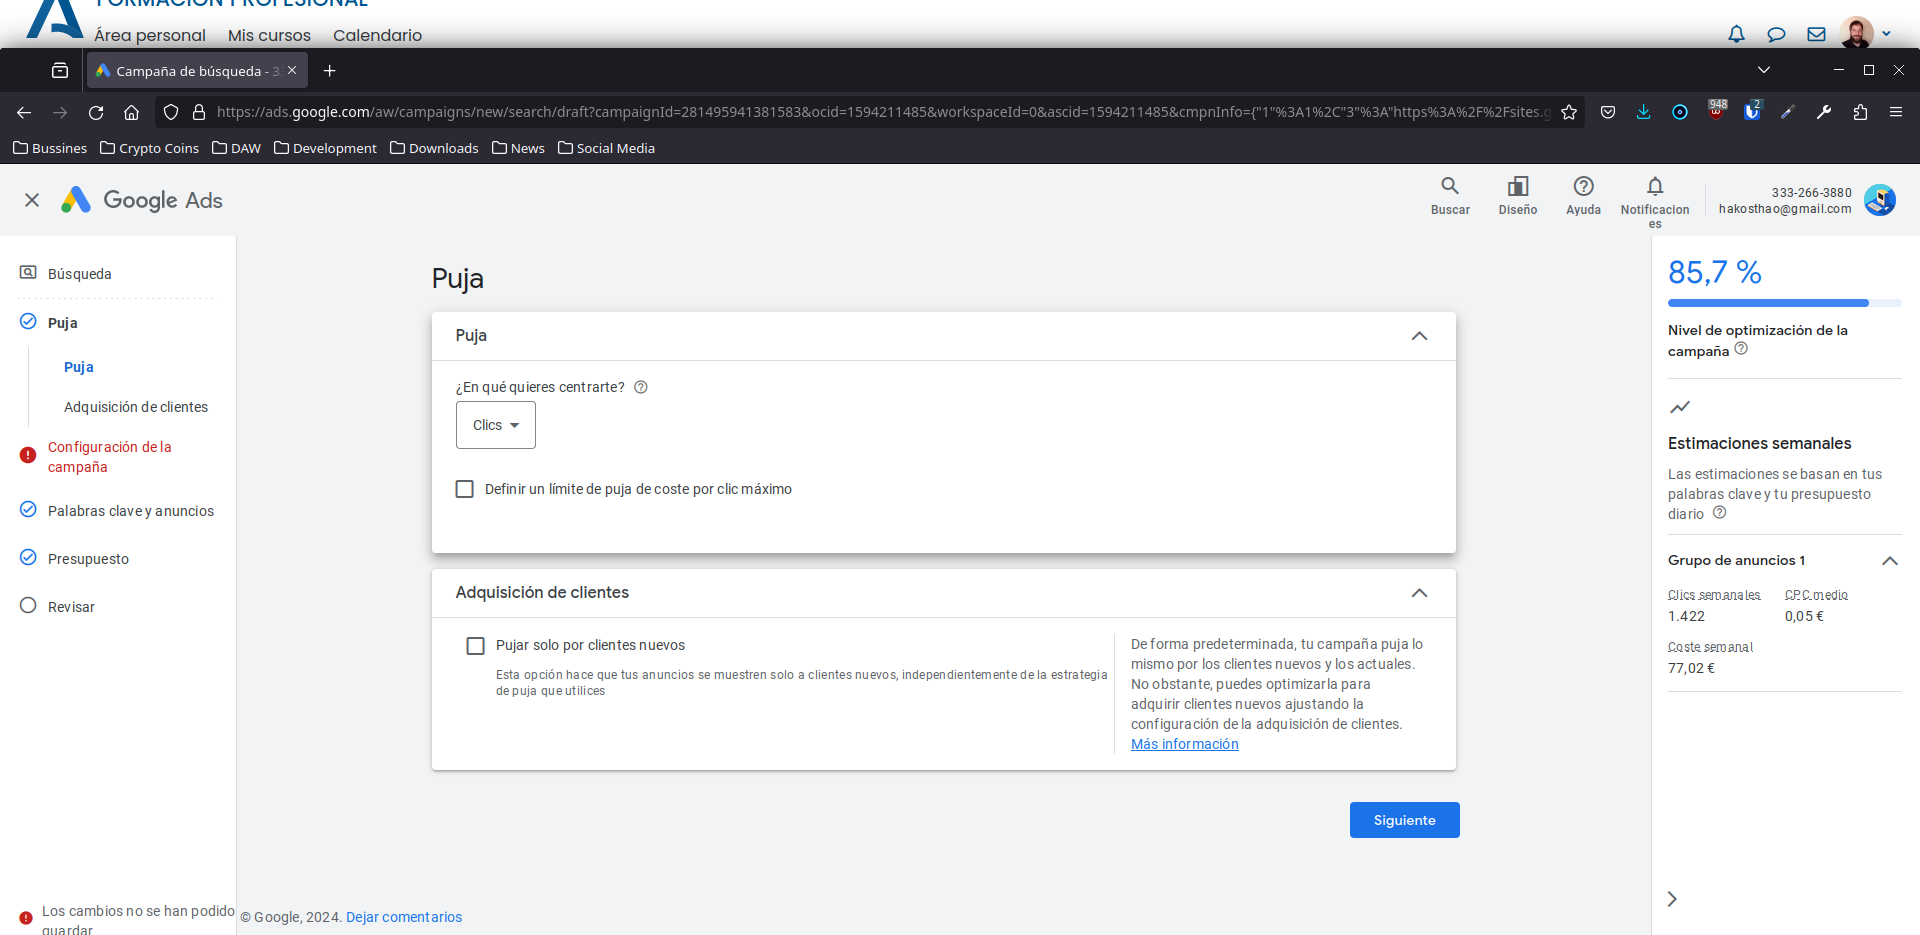
\includegraphics[scale=0.28]{Campana-clic.png}
        \caption{Selección del método de puja}
    \end{figure}

     \item Pulsando en siguiente, se nos mostrará una pantalla donde además de mostrarnos la información que hemos introducido hasta ahora, se nos pedirá que seleccionemos la ubicación objetivo, que en nuestro caso es \textbf{Granada}. Además hemos seleccionado 2 idiomas, \textbf{Español} e \textbf{Inglés}, para llegar a más audiencia, como podemos ver en la siguiente imagen.

    \begin{figure}[H]
        \centering
        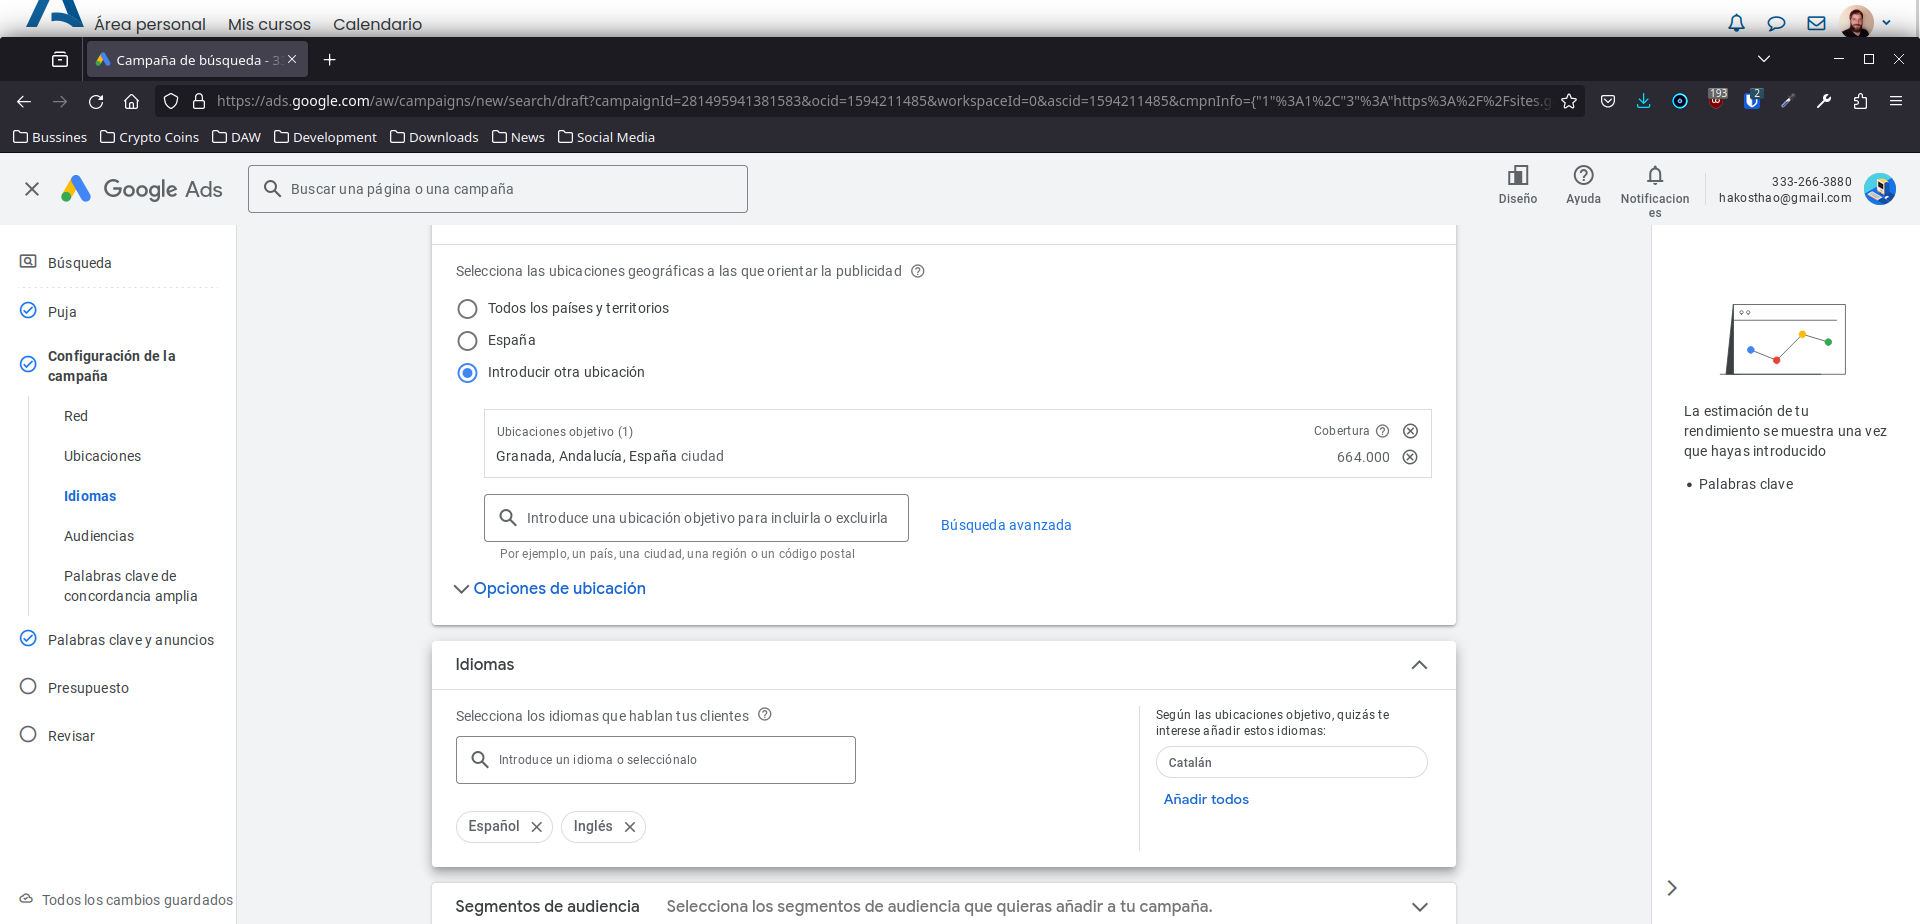
\includegraphics[scale=0.28]{Campana-ubi.png}
        \caption{Selección de ubicación e idioma}
    \end{figure}

    \item Pulsando en la opción de \textit{Más ajustes}, en esta misma página, se nos mostrarán formularios para introducir el horario, nosotros hemos seleccionado de \textbf{9:00 a 14:00} de \textbf{Lunes a Viernes} y de \textbf{11:00} a {19:00} los \textbf{Sábados y Domingos}. Además, hemos seleccionado como fecha de inicio, el \textbf{21 de Enero de 2024} y como fecha de final el \textbf{10 de Febrero de 2024}.

    Debíamos seleccionar el 10 de Enero, como indica el enunciado, pero ya que esta tarea la estoy realizando el 21 de Enero es imposible seleccionar esa fecha.

    \begin{figure}[H]
        \centering
        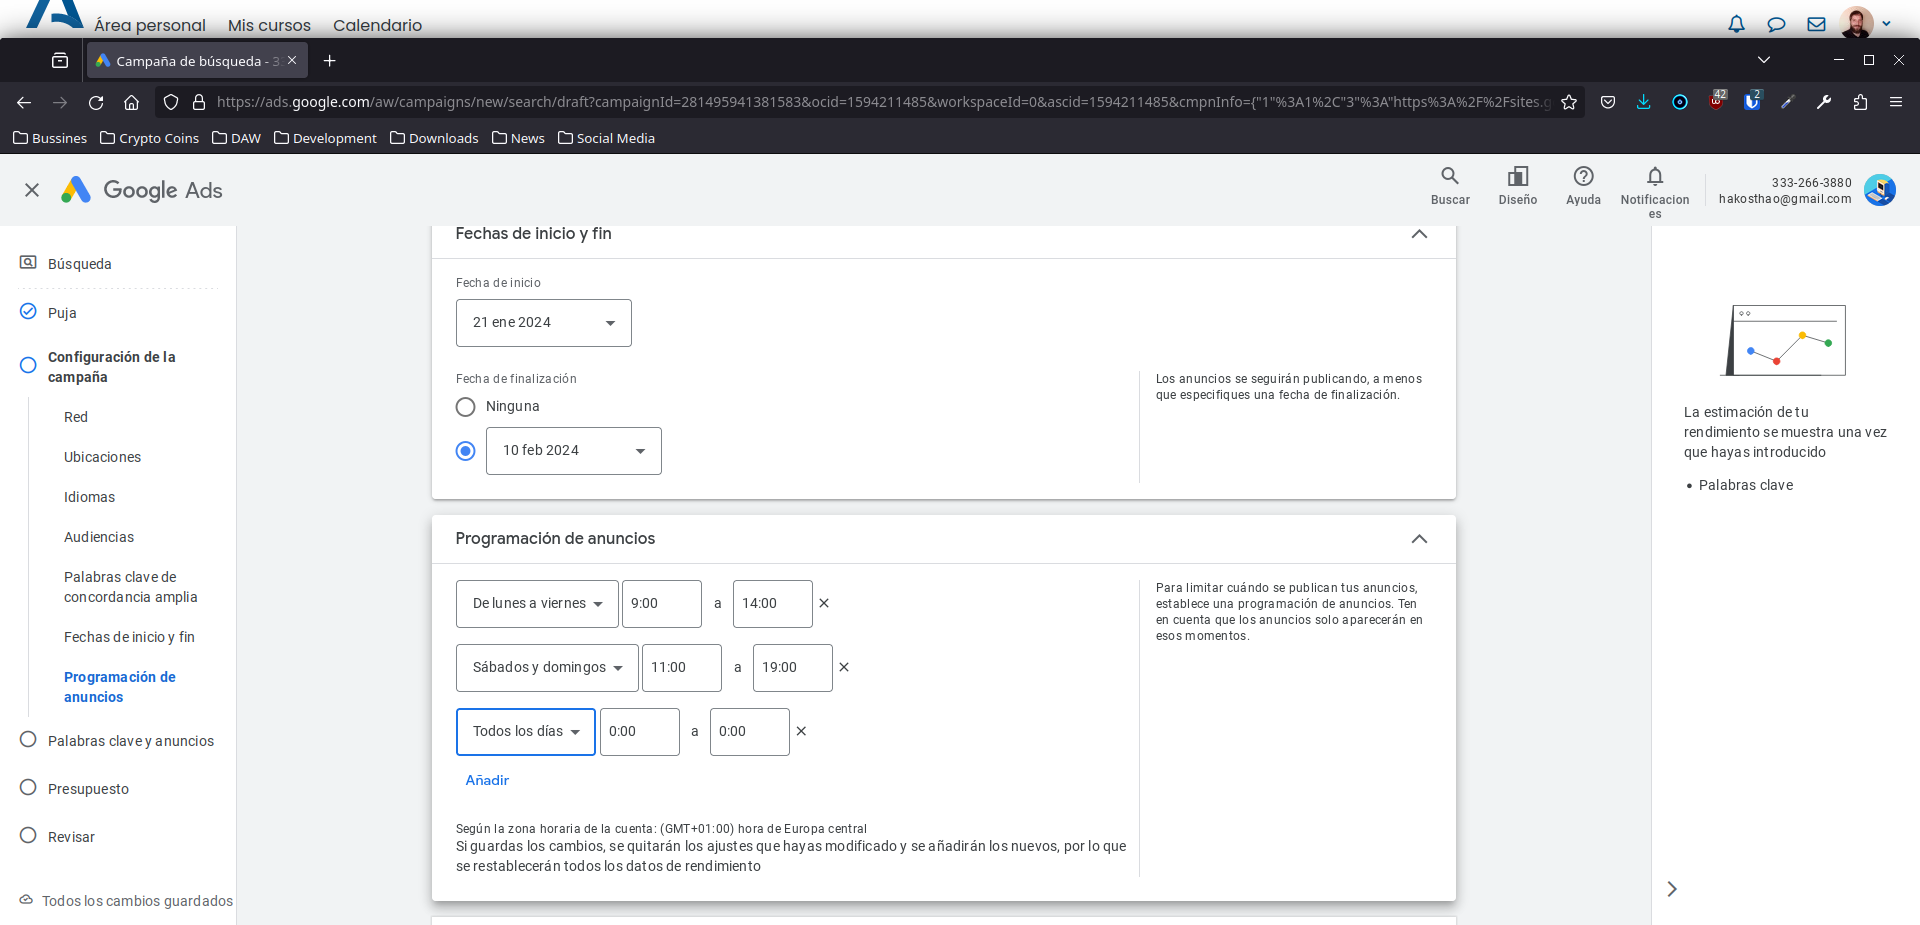
\includegraphics[scale=0.28]{Campana-fecha.png}
        \caption{Selección de fecha y horario de la campaña}
    \end{figure}

    \item En el siguiente punto, tenemos que seleccionar varias palabras clave para que nuestro anuncio se muestre. Hemos seleccionado 2 de las que nos sugería Google, estas son \textbf{web site google} y \textbf{web para empresas}. Además hemos añadido las 4 que habíamos seleccionado nosotros, es decir, \textbf{desarrollo web}, \textbf{diseño web}, \textbf{e-commerce} y \textbf{programador web en Granada}.

    Seleccionando la \textbf{concordancia amplia}, para la mayoría de palabras, así si un usuario buscar los términos web site google, web para empresas, diseño web o e-commerce, mezclados con otros terminos, usando plurales o sinónimos, nuestro anuncio se mostrará.

    Hemos seleccionado la \textbf{concordancia de frase} para el termino \textbf{"programador web en Granada"}, ya que es una palabra más específica y nos interesa que las búsquedas que incluyan este termino con alguno más agregado hagan saltar nuestro anuncio.

    También hemos seleccionado la \textbf{concordancia exacta} para desarrollo web, para que cada vez que se busque este termino exacto se muestres nuestro anuncio.

    \begin{figure}[H]
        \centering
        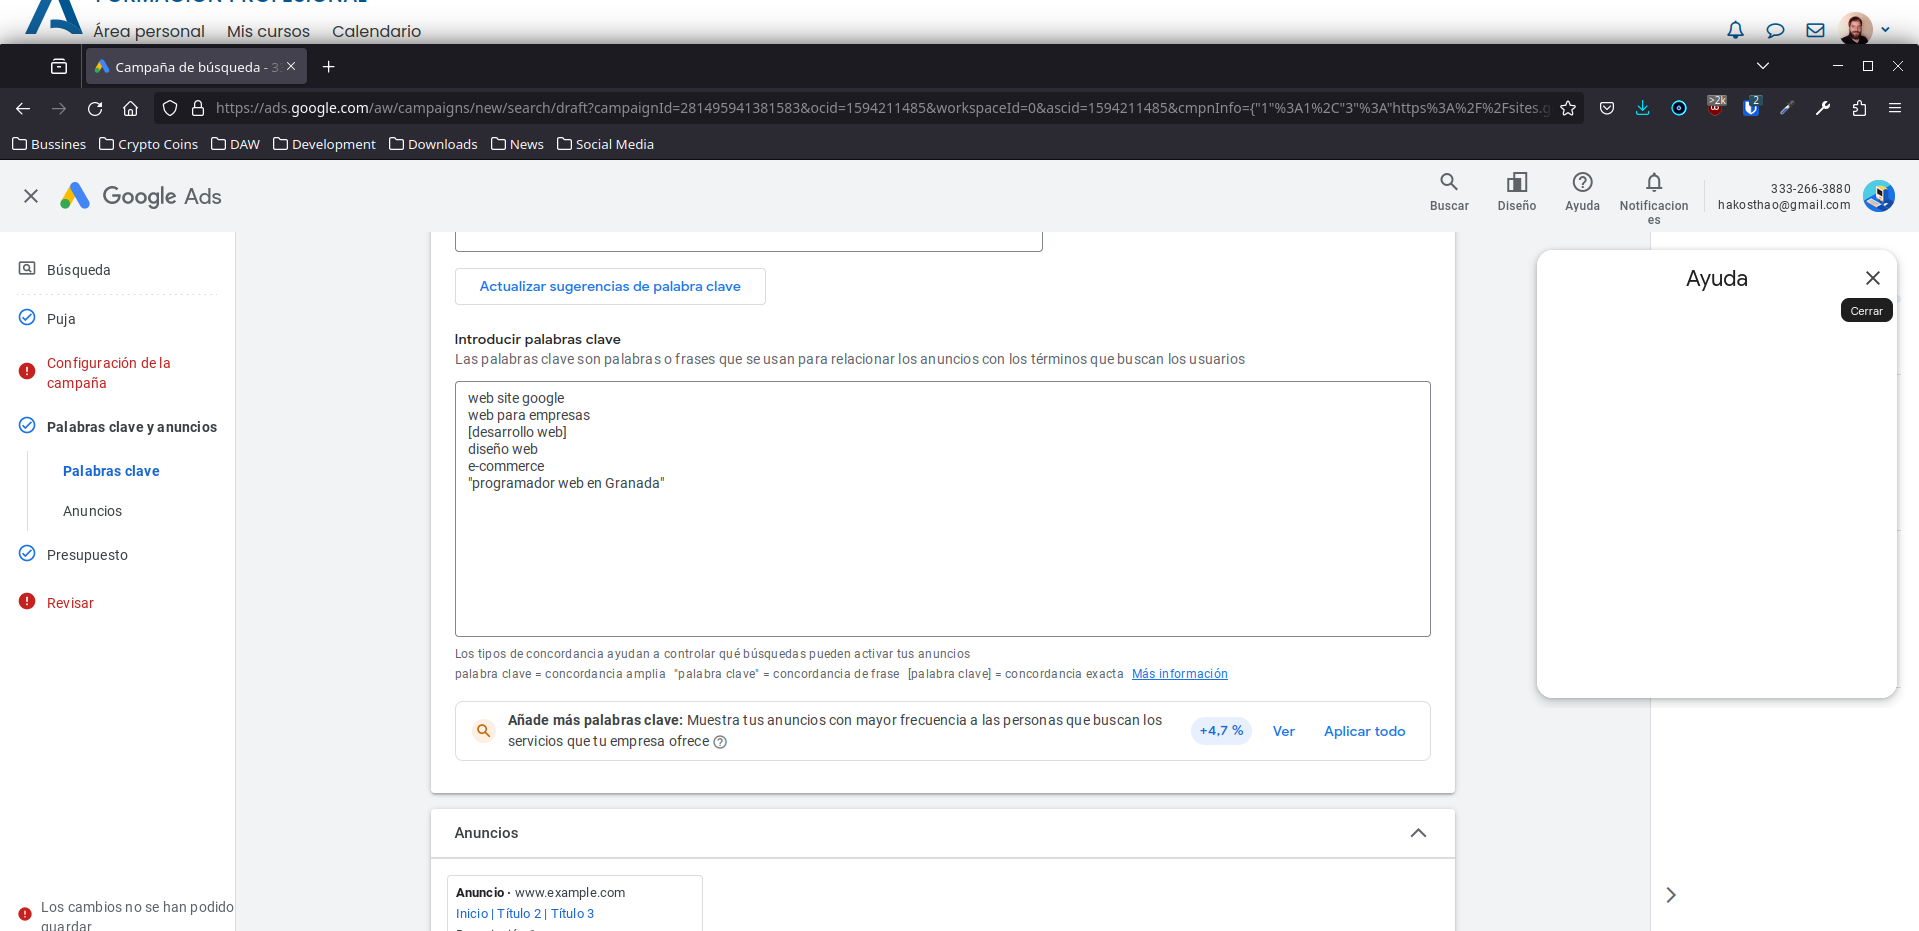
\includegraphics[scale=0.28]{Campana-palabras.png}
        \caption{Selección de las palabras clave}
    \end{figure}
\end{enumerate}

\section{Ejercicio 3}

\subsection{Enunciado}
Creación del anuncio:

\begin{itemize}
    \item Crea 3 títulos diferentes para el anuncio.
    \item Añade dos descripciones del mismo.
    \item Crea una extensión de enlace de sitio.
    \item Añade un numero de teléfono ( inventado), ( sección más recursos)

    \begin{itemize}
        \item CPC máx 0,15 €.
        \item Presupuesto diario 11€ ¿ qué clics semanales, cpc medio y coste semanal se estima?
    \end{itemize}
 \end{itemize}

\subsection{Solución}
Por últimos, vamos a crear una anuncio y a establecer el presupuesto para nuestra campaña. Para ello, hemos realizado los siguientes pasos:

\begin{enumerate}
    \item En la página que nos encontrábamos antes, hemos en la sección de anuncios, hemos pulsado en crear nuevo anuncio.
          Esto nos desplegará una pantalla donde podemos introducir todas las opciones de configuración de nuestro anuncio.
          Nosotros hemos añadido 3 títulos y 2 descripciones al anuncio para que se muestre a los usuarios.

          Los títulos han sido: \textbf{Pon tu negocio en la Red}, \textbf{Desarrollos Web a Medida} y \textbf{Desarrollos Web en Granada}.

          Mientras que las descripciones han sido: \textbf{Creación de páginas web a medida por precios asequibles} y \textbf{Pon tu negocio en la red y obten todos los beneficios de forma rápida}.

          En la siguiente captura vemos la introducción de esta información:

          \begin{figure}[H]
              \centering
              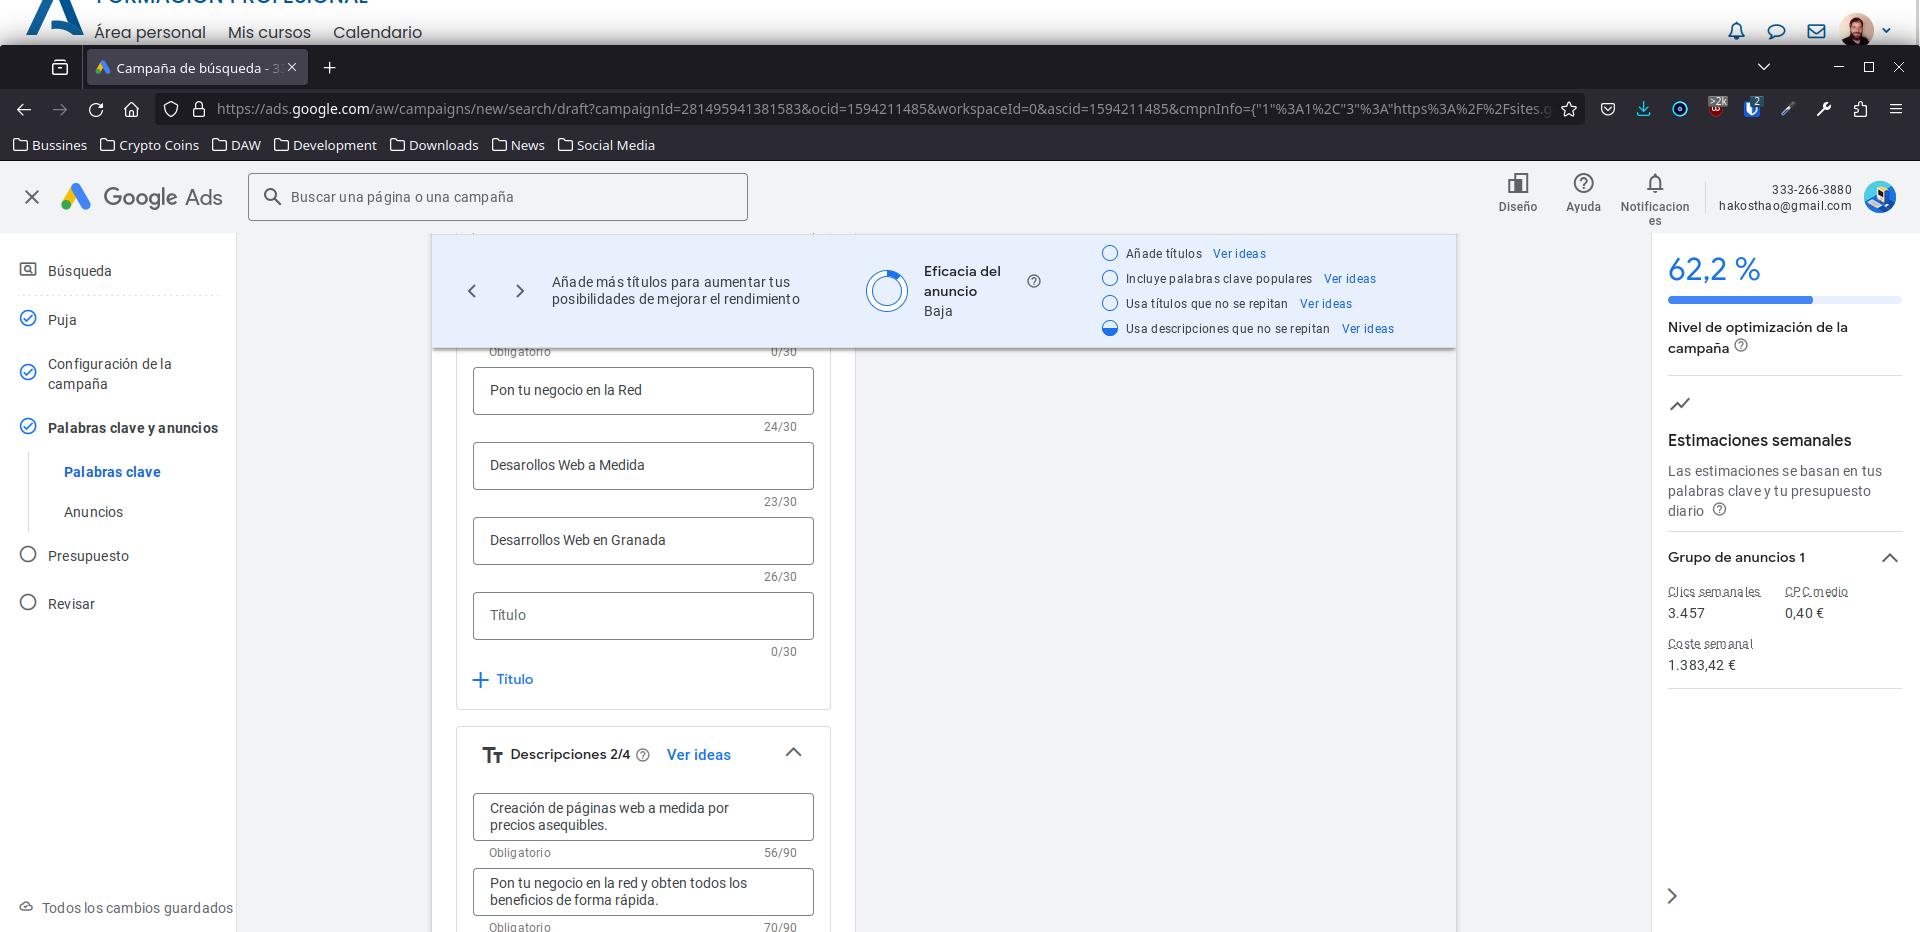
\includegraphics[scale=0.28]{Campana-anuncio.png}
              \caption{Configuración del anuncio}
          \end{figure}

      \item A continuación en la sección \textit{Mas Recursos}, hemos añadido un teléfono para que puedan contactar con nosotros, como vemos en esta imagen.

      \begin{figure}[H]
          \centering
          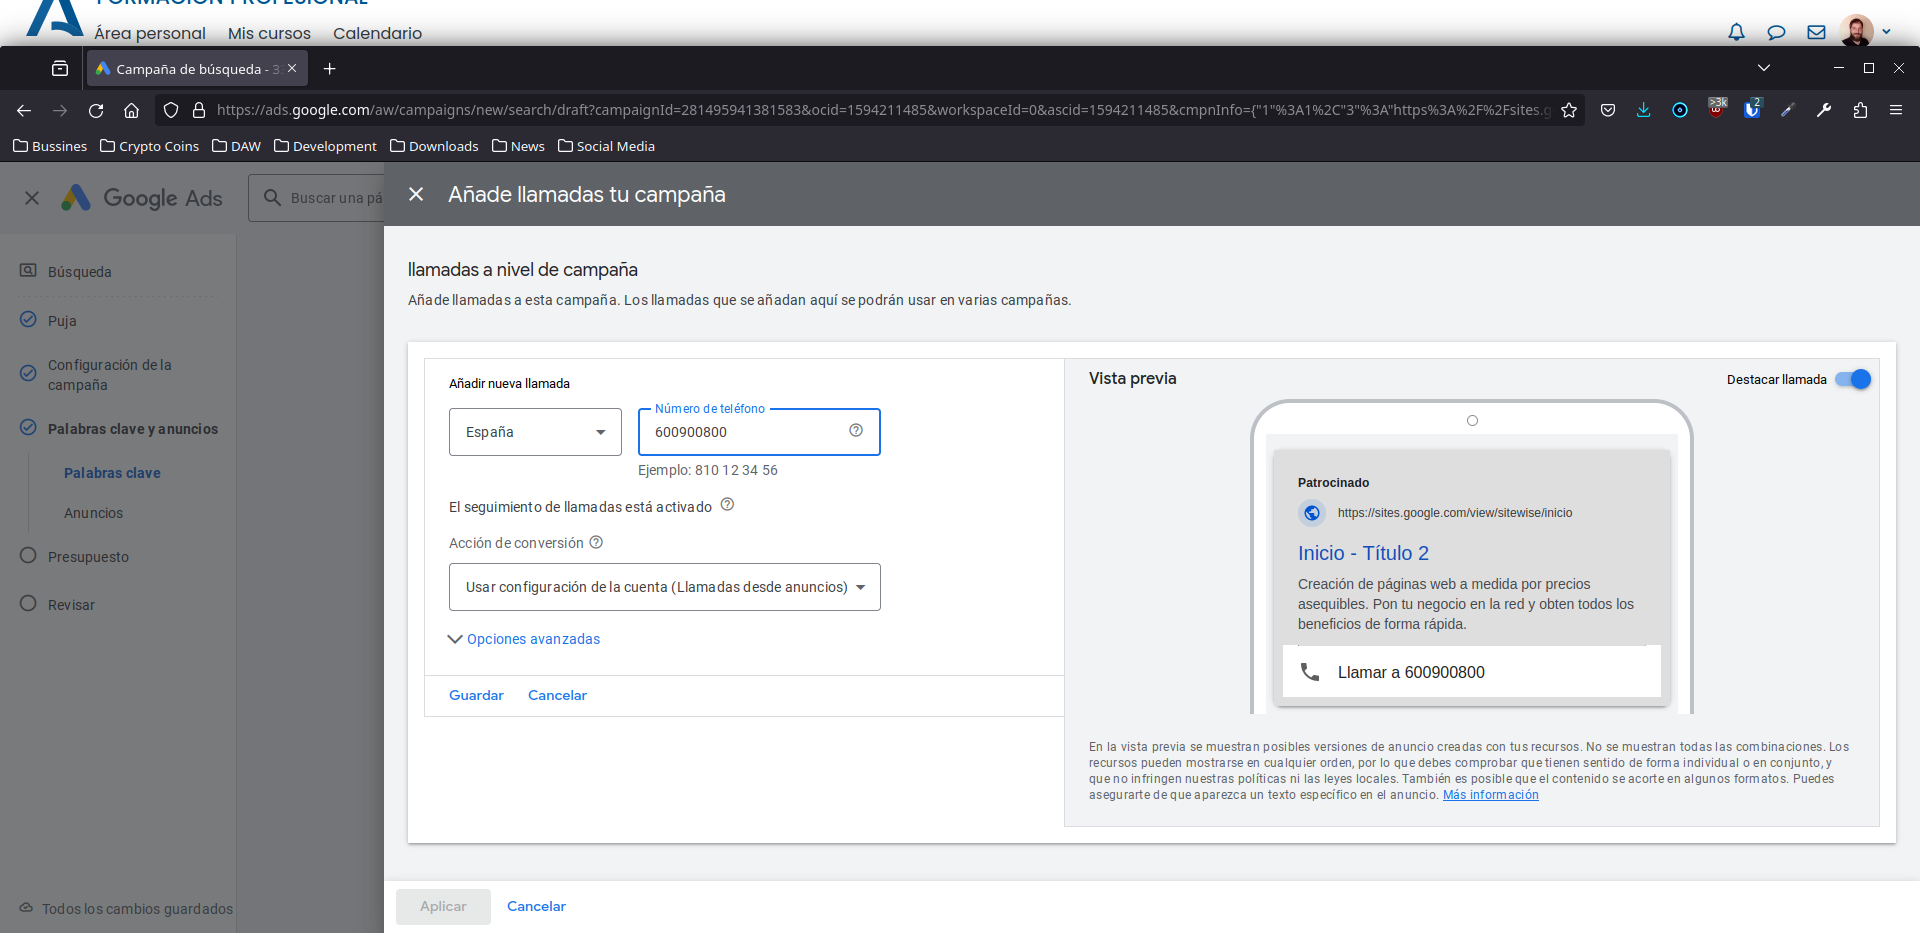
\includegraphics[scale=0.28]{Campana-tele.png}
          \caption{Introducción del teléfono}
      \end{figure}

      \item Por últimos, hemos creado nuestro presupuesto. Se ha establecido el presupuesto diario en \textbf{11€}, lo que ha dado como resultado los siguientes datos para los clics:

      \begin{itemize}
          \item Clics semanales: \textbf{827}
          \item CPC Medio: \textbf{0,09€};
          \item Coste Semanal: \textbf{77€}
      \end{itemize}

      En la siguiente captura podemos ver todos los datos introducidos así como la estimación de clics y su coste.

      \begin{figure}[H]
          \centering
          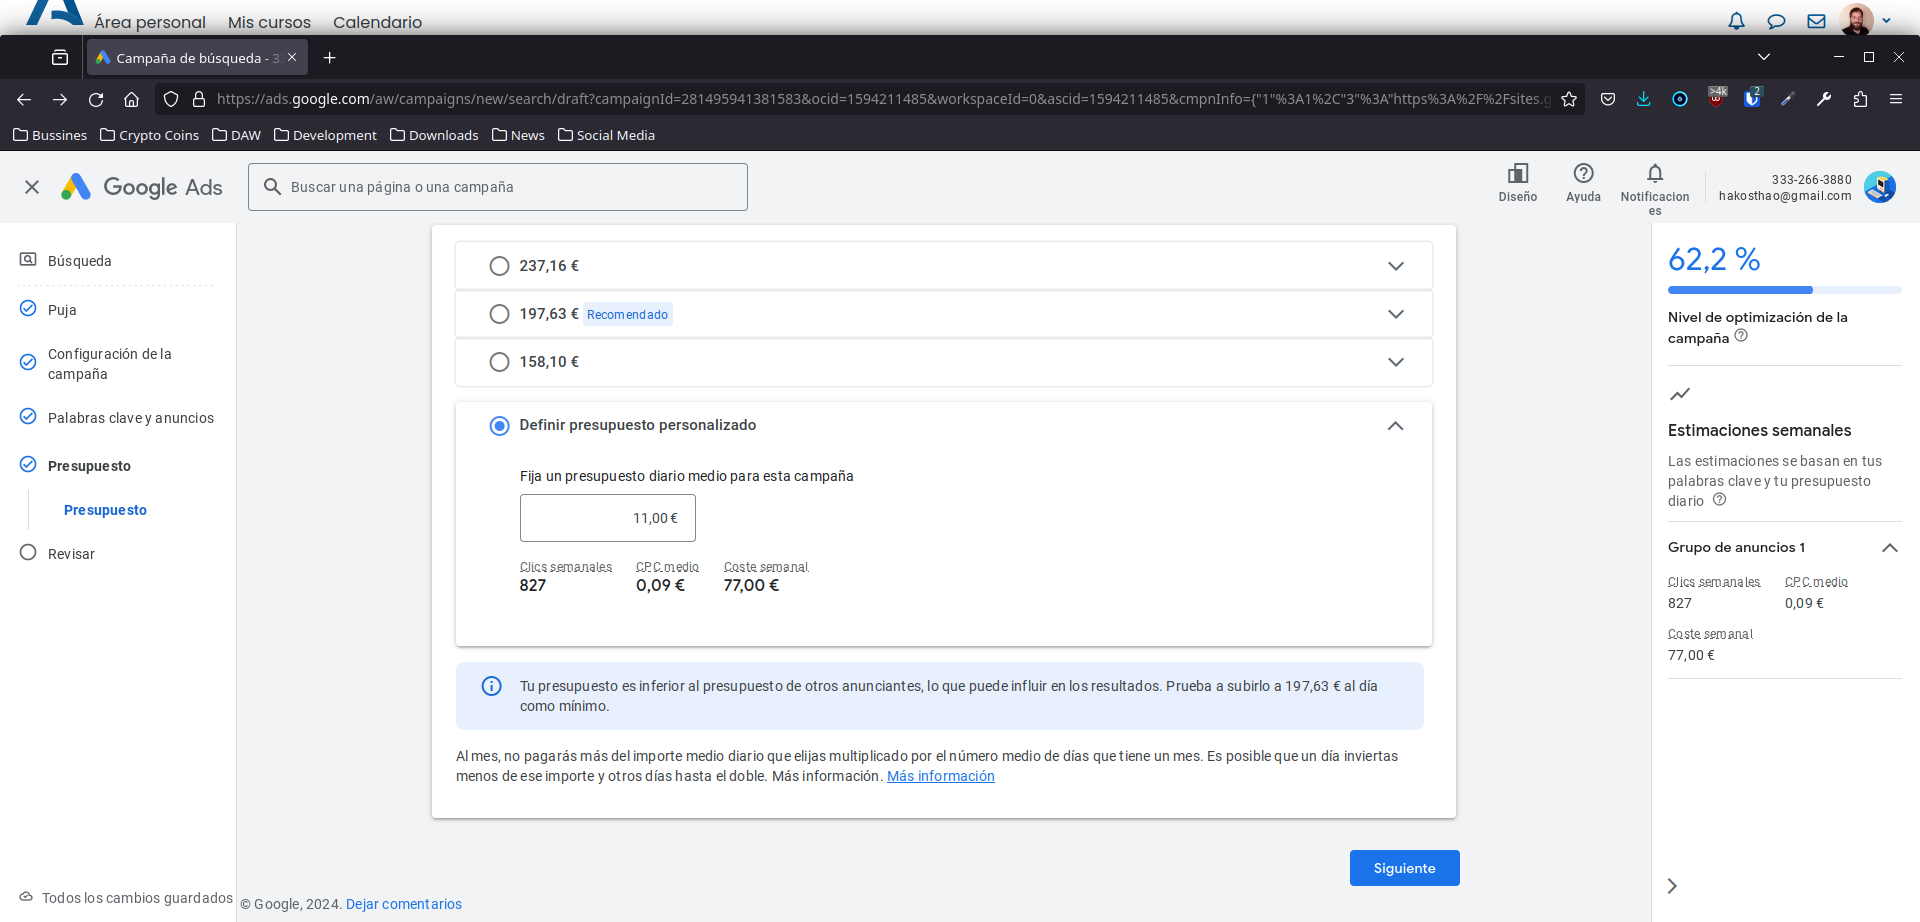
\includegraphics[scale=0.28]{Campana-presupuesto.png}
          \caption{Configuración del presupuesto}
      \end{figure}

      \item Tras pulsar en siguiente, la web comprobará que todos los datos están introducidos correctamente y la campaña quedará lista para publicarse, como se puede ver en la siguiente pantalla.

      \begin{figure}[H]
          \centering
          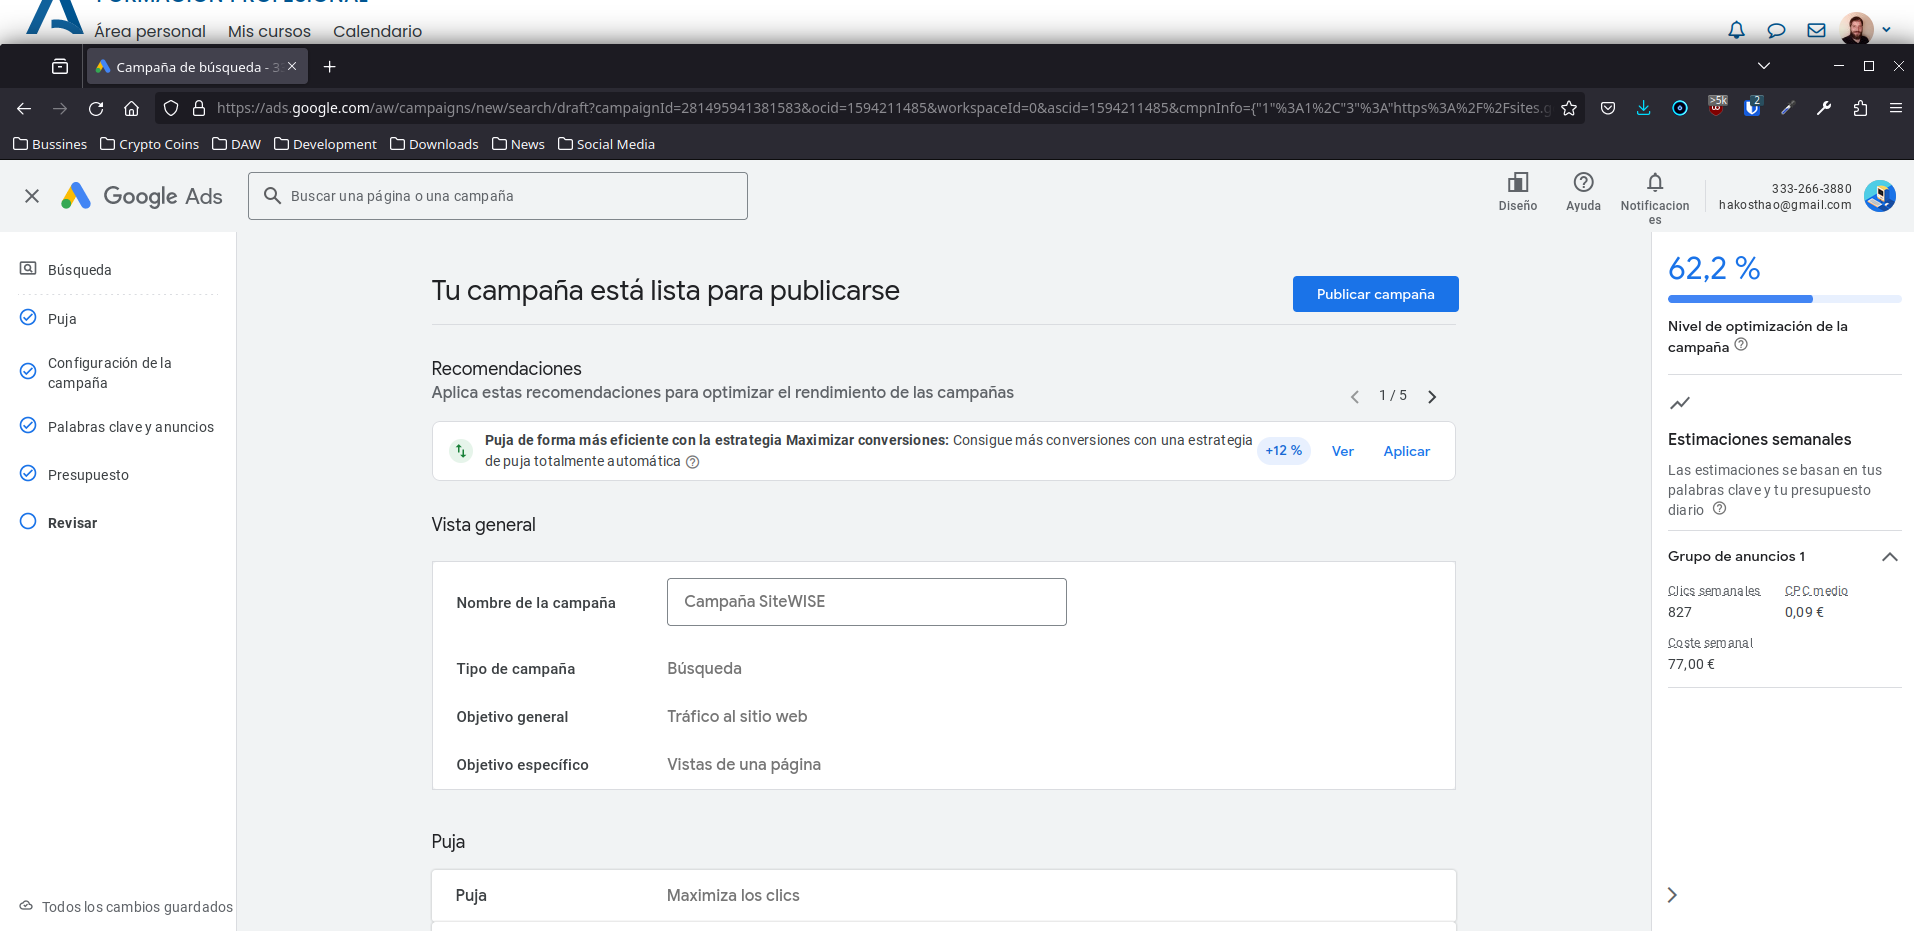
\includegraphics[scale=0.28]{Campana-publi.png}
          \caption{Campaña lista para publicación}
      \end{figure}
\end{enumerate}

\section{Ejercicio 4}
\subsection{Enunciado}
Realiza una aportación en el foro conclusiones de la tarea, indicando las dificultades que has encontrado y las mejoras que realizarías en la tare, así como si te ha parecido adecuada la tarea que se te ha pedido.

\subsection{Solución}
Se ha realizado el aporte al foro como se pedía en esta actividad y se incluye una captura de dicha información en la siguiente la imagen.

\begin{figure}[H]
    \centering
    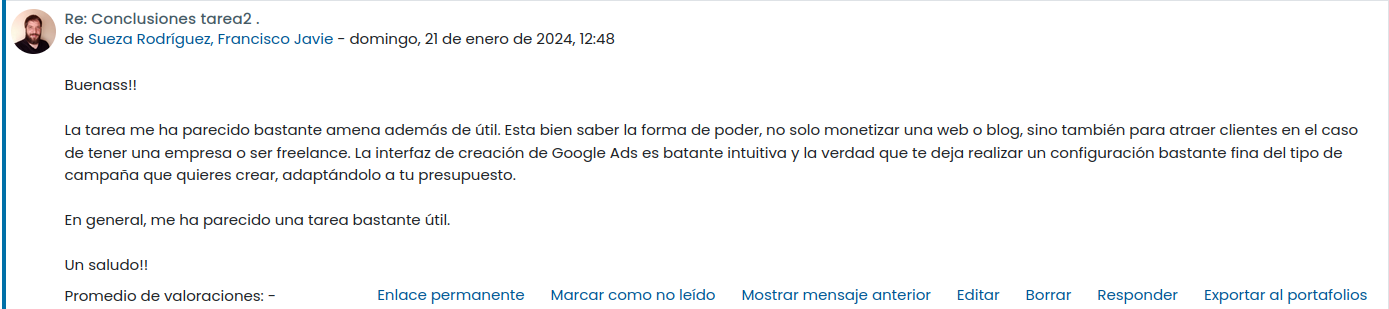
\includegraphics[scale=0.40]{apota-foro.png}
    \caption{Aportación al foro}
\end{figure}

% Bibliography

%\newpage
%\bibliography{citas}
%\bibliographystyle{unsrt}

\end{document}